\chapter{Implementation}
This chapter will describe how the implementation for the evaluation has been made. first lets take a look at what has to be implemented and why.
\begin{itemize}
\item Test Level\\
this is the 3D environment that will be used to test the different control schemes. 
\item Gyroscopic controls\\
The control scheme that will use the gyroscope found in many mobile devices, what the gyroscope will be used for is to make it seem natural to turn around when looking in a virtual 3D space environment. 
\item Joystick controls\\
this control scheme is composed of two joystick like buttons, that respond to being dragged, one joystick will control the camera movement and the other the orientation of the camera. The idea is that this control scheme will seem familiar%reference to UX section
to users because the common place console controller uses the same kind of dragable joystick.
\item Standard button controls\\
Because the previously described control schemes uses concepts that might not be immediately familiar to all users, this standard button control scheme was designed to see if users who are not familiar with joysticks and using their body movements, would perform better with a control scheme made out of buttons, all the buttons are able to trigger when being held down.
\end{itemize}
these four things are what is needed in the projects implementation. To implement this what is needed is some sort of framework for working within a 3D environment, there are two ways to go about this, either build such a framework from scratch or use one of the many game engines available. Since developing a fully fletched 3d engine is beyond the scope of this project, the choice fell on developing from within an available 3D engine

\subsection{Implementation of 3D testing area}
To test different non-traditional control schemes 3D test area was created. It consists of twisted path that test participants had to walk through as fast as possible.
\begin{figure}[H]
\centering
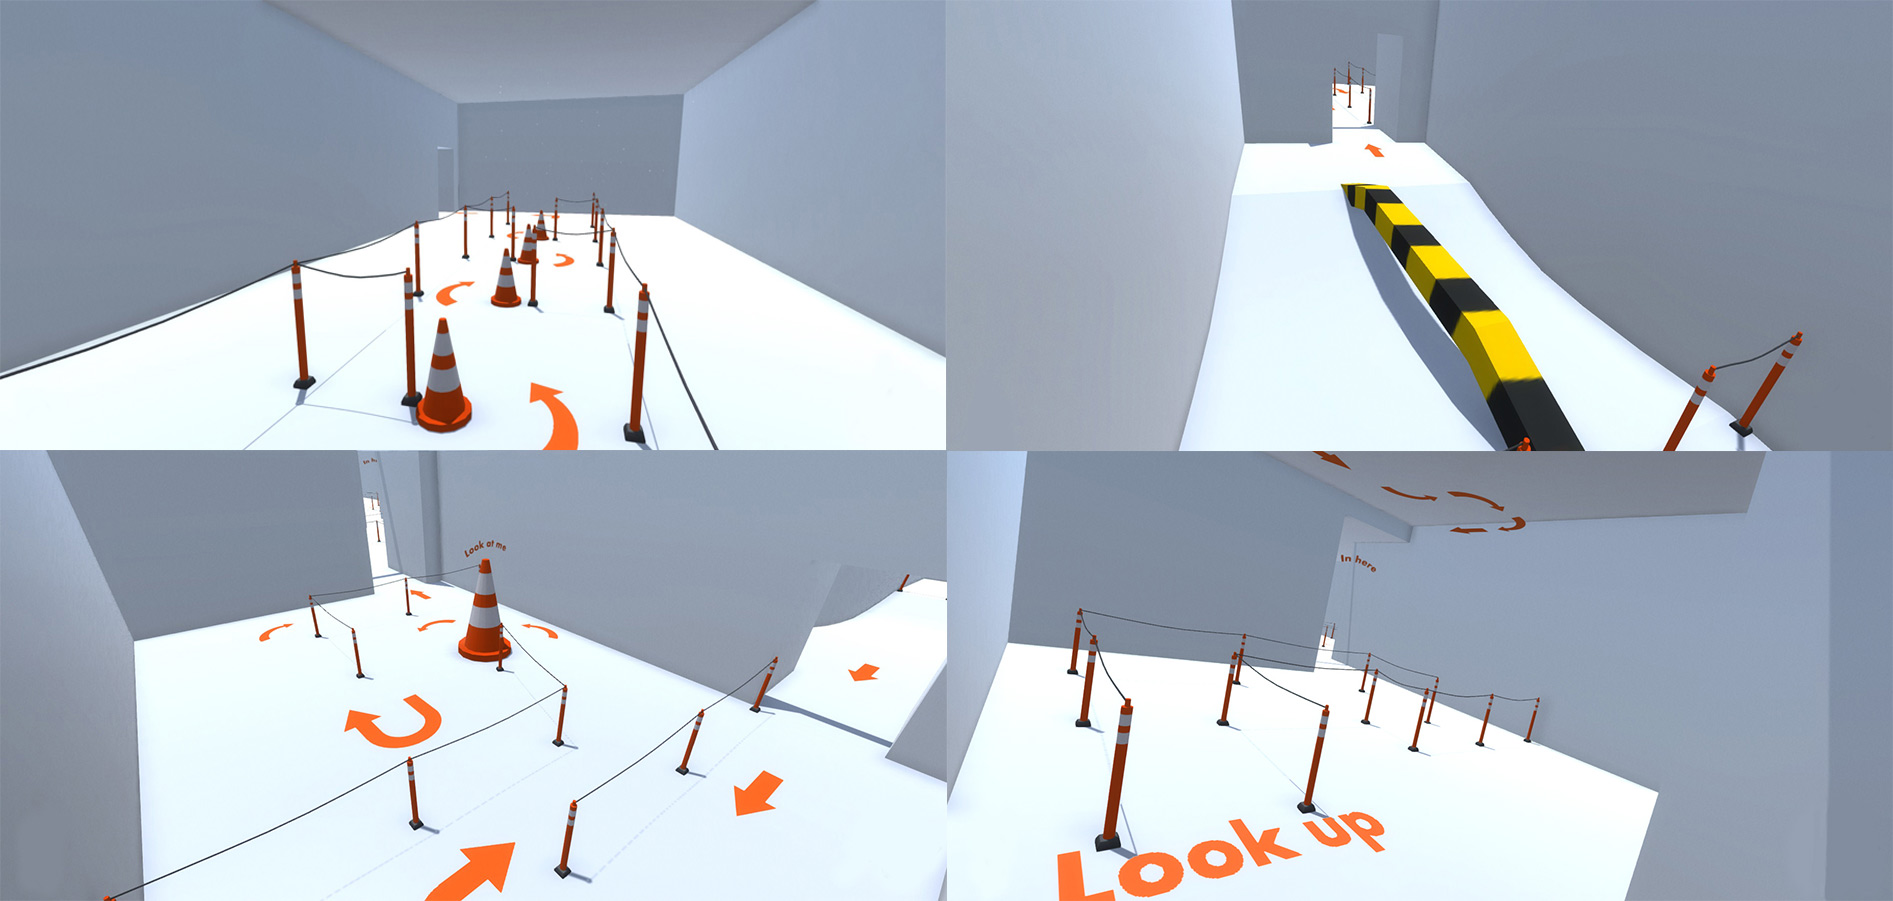
\includegraphics[scale=0.26]{3D_dev_6.jpg}
\caption{Pictures of the testing area}
\end{figure}

Focus of testing area was only on navigation for different schemes, so effort was placed on path and tasks and not on environment itself. All not important bits of the area were colored white and important as navigational arrows, cones and poles, explanatory text notes colored with sharp contrasting colors as red and orange. 

Analysing SOTA’s applications gave understanding what important aspects of navigation is. Firstly walking fluently around obstacles as furniture, doors, narrow paths. First two levels were developed for this to test. Second consideration was that users need to look around placed furniture which was not considered in most SOTA analyzed applications. Small area with huge cone and text “look at me” was placed and arrows in circular path around it. This represents how user would walk around furniture and inspect it by looking - focusing on one point while walking around. Next two levels were developed to test how efficient it is to look up and down while walking in given direction. it represents looking at the lamp, carpet or any other element that is placed above or below user. The last test area was created to see how user goes straight but looks to one side as the user would walk-by, but focus at some furniture aside.
\begin{figure}[H]
\centering
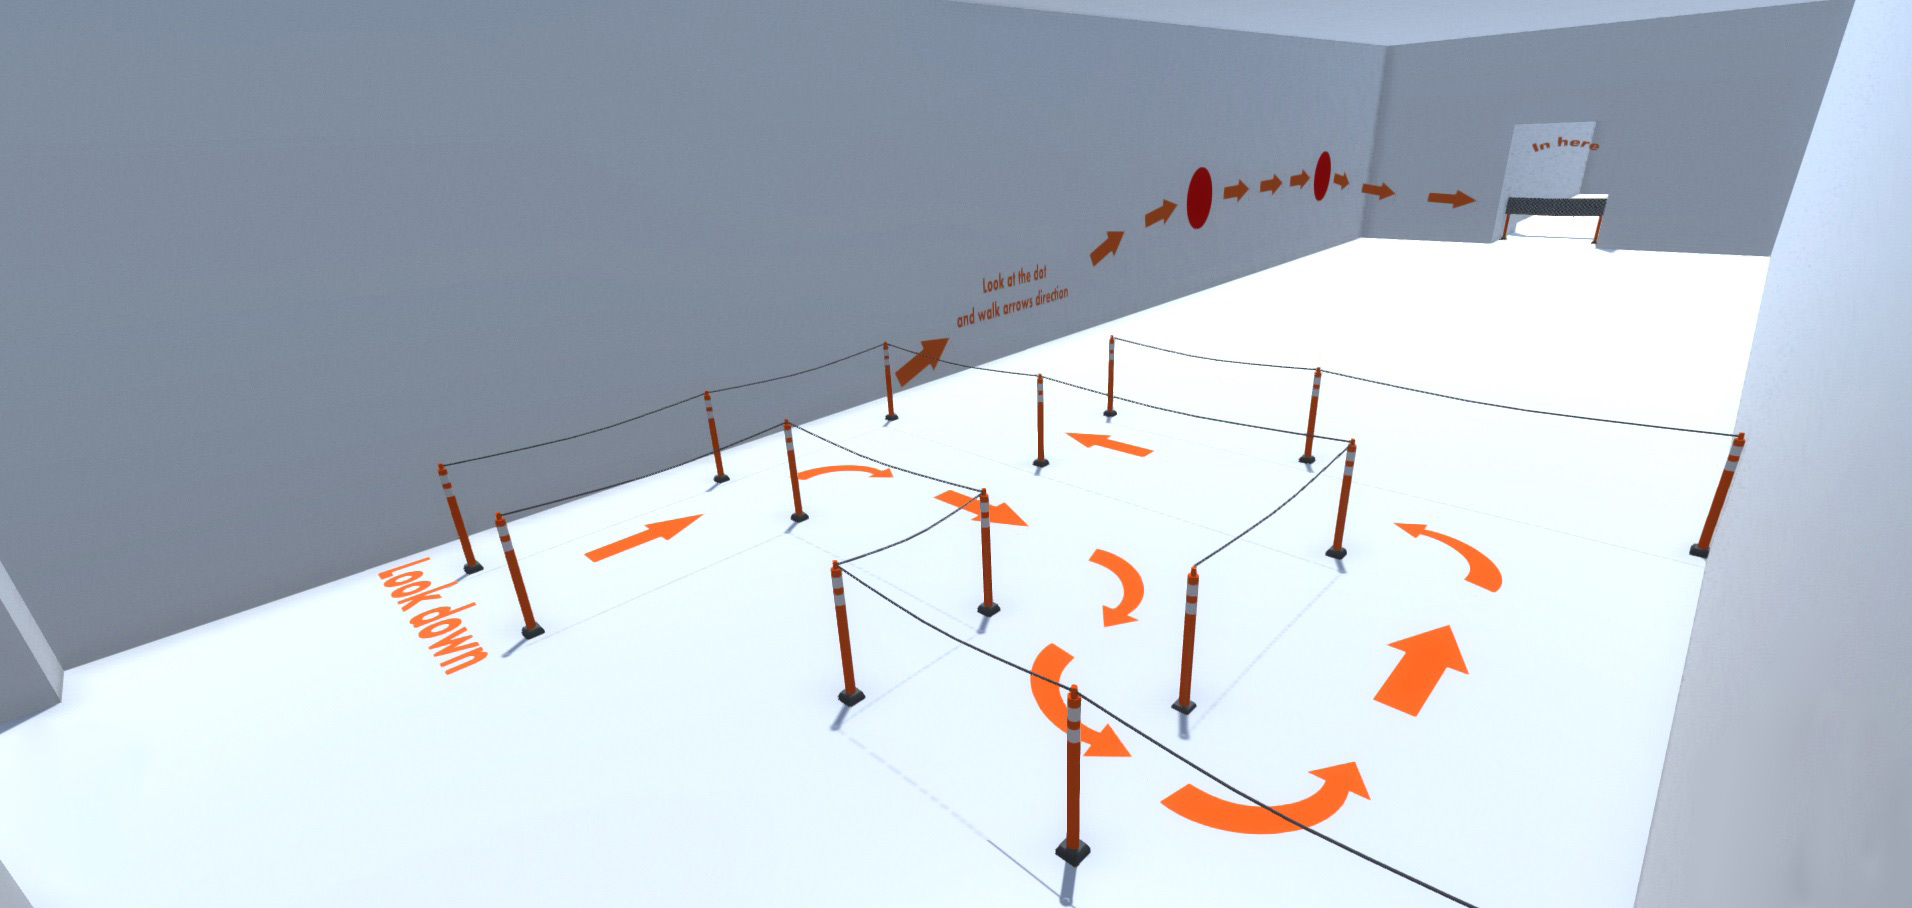
\includegraphics[scale=0.25]{3D_dev_5.jpg}
\caption{Last level of testing area. This level is to test how well user can walk while looking down and sideways}
\end{figure}

\subsubsection{Development of 3D elements}
Actual implementation consisted of creating level areas, 3D prefabs - cones and poles with string, sprites - notes and arrows. 3D elements were created using software “Maya” and textures with “Photoshop”. Each level started by simple creation of a square representing a room. Then considerations of what test it will include were done and assets that were created were placed making different challenges. Picture bellow shows 3D cone and it’s texture. 
\begin{figure}[H]
\centering
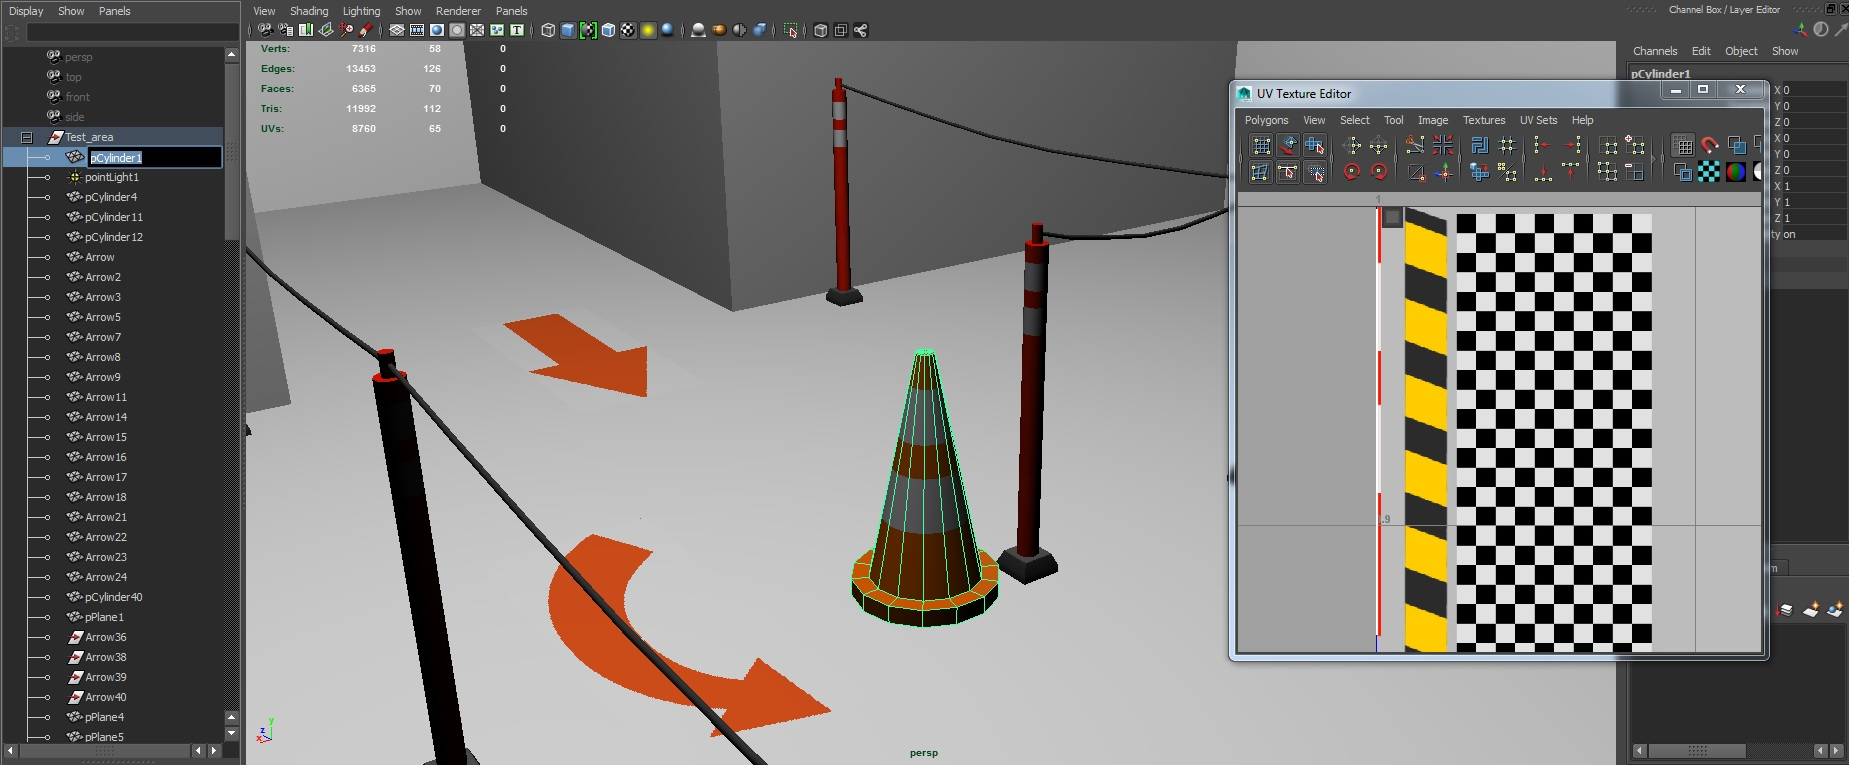
\includegraphics[scale=0.35]{3D_dev_7.jpg}
\caption{picture of a cone from testing level}
\end{figure}

Every object that required texturing, also needed its own UV map. UV map is 3 dimensional model representation in 2 dimensions - it helps to see and paint texture using tools as Photoshop. Since graphics and aesthetics were not focus of this test level, textures were created very minimalistic - without any shadowing, noise, imitation of being old or used etc. It also helped to make test very optimized in hardware performance, since textures size on disk were as little as few kilobytes. 


